\documentclass[a4paper,12pt]{report}
\renewcommand\thechapter{\Roman{chapter}}
\usepackage[utf8]{inputenc}
\usepackage{lipsum}
\usepackage{kantlipsum}
\usepackage[calcwidth]{titlesec}
\usepackage{fix-cm} 
\usepackage[Sonny]{fncychap}
\usepackage{setspace}
\usepackage{natbib}
\usepackage{pdflscape}
\usepackage{float}
\usepackage{siunitx,booktabs}
\usepackage{pgfplotstable}
\usepackage{pgfplots}
\usepackage{subcaption}
\usepackage{lscape}
\usepackage{graphicx}
\usepackage[raggedrightboxes]{ragged2e}
\usepackage{changepage}
\usepackage{makecell}
%\usepackage{biblatex}
%\addbibresource{references.bib}
%\bibliographystyle{apacite}

\usepackage{lipsum}% For 'Lorem Ipsum' dummy text
\usepackage[pscoord]{eso-pic}% The zero point of the coordinate systemis the lower left corner of the page (the default).

\newcommand{\placetextbox}[3]{% \placetextbox{<horizontal pos>}{<vertical pos>}{<stuff>}
  \setbox0=\hbox{#3}% Put <stuff> in a box
  \AddToShipoutPictureFG*{% Add <stuff> to current page foreground
    \put(\LenToUnit{#1\paperwidth},\LenToUnit{#2\paperheight}){\vtop{{\null}\makebox[0pt][c]{#3}}}%
  }%
}%

\pgfplotsset{
        compat=1.3,
    }
\pgfplotsset{compat=newest}
\usetikzlibrary{patterns}
\usepgfplotslibrary{fillbetween}
\sisetup{group-digits=false}

\doublespacing
\setlength{\parindent}{0pt}
\renewcommand{\baselinestretch}{1.3} 

\titleformat{\chapter}[display]{\Large}{\centering
  \MakeUppercase{\chaptername}\quad{\Huge\thechapter}}{10pt}{\titlerule[.5pt]\vspace{10pt}\centering
  \MakeUppercase}[\vspace{10pt}{\titlerule[.5pt]}]% <-- spacing of title bar
\titlespacing{\chapter}{0pt}{-80pt}{1cm}% <-- spacing of title bar


\usepackage{amsthm, amsmath, amssymb, mathtools, mathbbol}
\numberwithin{equation}{section}
\theoremstyle{definition}
\newtheorem{thm}{Theorem}[section]
\newtheorem{Def}[thm]{Definition}
\newtheorem{prob}[thm]{Problem}
\newtheorem{rem}[thm]{Remark}

%\usepackage{natbib}
\usepackage{graphicx}

\graphicspath{{graphics/}}

\begin{document}


\begin{center}

\Large NATIONAL UNIVERSITY OF SINGAPORE\\ 
\Large Master's of Computing (General-Track) \\ [0.2in]

\includegraphics[width=10cm]{1.nus_logo_full-horizontal} \\
\Large {\bf Alpha Tree Search and Machine Learning Approaches to Optimising Real Estate Portfolios}\\ [0.2in]
Leong Wei Ming \\
Supervisor: Professor Liu Li Li \\
Examiner: Professor Chin Wei Ngan \\ [0.3in]
Department of Computer Science \\
Internal Capstone Project for AY2023/2024
\end{center}

\chapter*{Abstract}
An internal project about applying genetic algorithm to search for optimal alphas.    
State the major contribution:

\chapter*{Declaration}
\begin{center}{\large
I hereby declare that this project report is my original work and it has been written by me in its entirety. I have duly acknowledged all the sources of information which have been used in this report. \\[0.5in]
This report has also not been submitted for any degree in any university previously.
}

\chapter*{Acknowledgement}
{\large
I would like to thank Professor Liu Lili for her guidance, support and encouragement throughout the course of this project. Working with Professor Lili has been a great learning experience, getting to learn much more about machine learning and its applications to finance in solving some challenges faced by industry practitioners. \\[0.5in]
Also many thanks to Professor Chin Wei Ngan for taking the time out to assess this project.

}
\end{center}
\setcounter{secnumdepth}{3}
\setcounter{tocdepth}{3}

\tableofcontents

\setcounter{chapter}{1}
\renewcommand{\thechapter}{\arabic{chapter}}
\pagenumbering{arabic}
\setcounter{chapter}{0}
\chapter{Introduction}
The saying goes that once a profitable trading formula has been discovered and traded on by enough people, its profits will be eroded away and it will cease to be profitable. Traders and investors appear to be playing a never-ending game of "Hide-and-Seek" in search of profitable trading strategies. Due to the evolving nature of the financial markets, traditional financial time-series forecasting models which are static in nature are becoming less effective than Machine Learning models and dynamic algorithms in identifying the best investments \cite{sheth_predicting_2023}. The success of Machine Learning has led to numerous research papers applying a myriad of Machine Learning techniques to predict stock prices \cite{obthong_survey_2020}. However, fewer papers apply these approaches in the Real Estate sector and these papers largely focus on future stock price prediction rather than portfolio allocation as a whole \cite{habbab_-depth_2024}. Many of these papers also use price-volume data without fundamental financial data as inputs. In 2022, the global real estate sector was worth more than \$380 trillion and worth more than the global equity and bond markets combined \cite{tostevin_total_2023}, with approximately 893 listed Real Estate Investment Trusts (REITs) \cite{nareit_global_2024}. Hence, addressing the research gaps in this sector is particularly valuable.


\section{Problem Definition}
The aim of this report is to develop an effective real estate portfolio optimisation model that maximises profits, minimises risks and outperforms the market indexes with a sharpe ratio of more than 2. A novel approach of applying Genetic Algorithms to search for outperforming Alpha formulas, as well as, three Machine Learning models, namely, Multiple Linear Regression (MLR), Neural Networks (NN) and Long-Short Term Memory (LSTM) are used to construct models. A trading agent is also constructed to allocate funds to the portfolio based on the results from the models. The input data to the Machine Learning models will be extended beyond price-volume data to include fundamental stock data. The models will be trained on 10 years worth of real market data. Then, the performances of these approaches will be compared with traditional financial models and the market indexes.

\section{Motivations}
Interviews of traders and financial journalists have revealed that both technical and fundamental analysis are used for forecasting investments, for shorter and medium to long term investment horizons respectively \cite{oberlechner_importance_2001}. Given that most investments in real estate are meant for the medium to long term, the lack of fundamental data inputs for REITs stock price predictions reveals a pressing need for fundamental data to be incorporated. \\ 

In the field of quantitative trading, quant firms seek to develop predictive algorithms for quantitative trading called "Alphas" that determine how capital is allocated to portfolios profitably \cite{tulchinsky_finding_2019}. What began with investment experts manually constructing Alpha formulas has gradually been replaced with automated alpha mining techniques that employ Machine Learning algorithms \cite{wang_alpha-gpt_2023}. There appears to be an opportunity to apply the concept of quantitative finance Alphas for Real Estate portfolio allocation. In addition, researchers have been inspired by Charles Darwin's theory of evolution \cite{ruse_charles_1975} to develop a Genetic Algorithm and have applied it in finance \cite{aguilar-rivera_genetic_2015}. Synthesising these two ideas, presents a new and innovative approach to use Genetic Algorithms to search for Alphas in the Real Estate sector. \\

Lastly, as most of past research is centered on price prediction, there is a need to develop trade execution logic to allocate portfolios based on these predictions.



\section{Major Contributions and Creativity}
The first major contribution of this project is the analysis on REITs stock datasets with more than 150 features of technical and fundamental indicators. This expands the dimensionality of the input training data significantly beyond price-volume features to incorporate REIT company data from financial statements. The comprehensive dataset covers 150 out of the total worldwide population of 893 REITs and includes up to 20 years of historical data.\\

Creativity is demonstrated in the writing of a Genetic Search Algorithm that searches for outperforming REIT Alphas. It resulted in the second major contribution of a trading model with superior returns that significantly outperforms the market indexes.\\ 

The third contribution is the implementation of a trading agent or trade execution logic that acts on individual REIT price predictions to allocate funds to selected REITS in a portfolio.\\

Overall, this research paper has expanded the body of knowledge on the application of Alphas and Machine Learning models in Optimising Real Estate Portfolios.

\titleformat{\chapter}[block]
  {\normalfont\huge\bfseries}{\thechapter.}{1em}{\Huge\centering}
\titlespacing*{\chapter}{0pt}{150pt}{0pt}
\setcounter{chapter}{0}
\renewcommand{\thechapter}{\Roman{chapter}}
\chapter{Background}


\titleformat{\chapter}[display]{\Large}{\centering
  \MakeUppercase{\chaptername}\quad{\Huge\thechapter}}{10pt}{\titlerule[.5pt]\vspace{10pt}\centering
  \MakeUppercase}[\vspace{10pt}{\titlerule[.5pt]}]% <-- spacing of title bar
\titlespacing{\chapter}{0pt}{-80pt}{1cm}% <-- spacing of title bar
\renewcommand{\thechapter}{\arabic{chapter}}

\pagenumbering{arabic}
\chapter{Financial Terminology and Concepts}
In order to better communicate ideas, the key financial terminologies and formulas will be explained. Particularly the difference between a stock, REIT and a portfolio, the difference between technical and fundamental analysis and the concept of Alphas. This builds the foundation for further discussions on the measures of portfolio performance, namely, profits/losses and the sharpe ratio. Other methods of analysis such as sentiment and macro-economic analysis is also briefly discussed. 
\section{Key Terms}
The relationship between stocks, REITs and Portfolios can be illustrated in the figure below.
\begin{figure}[H]
  \centerline{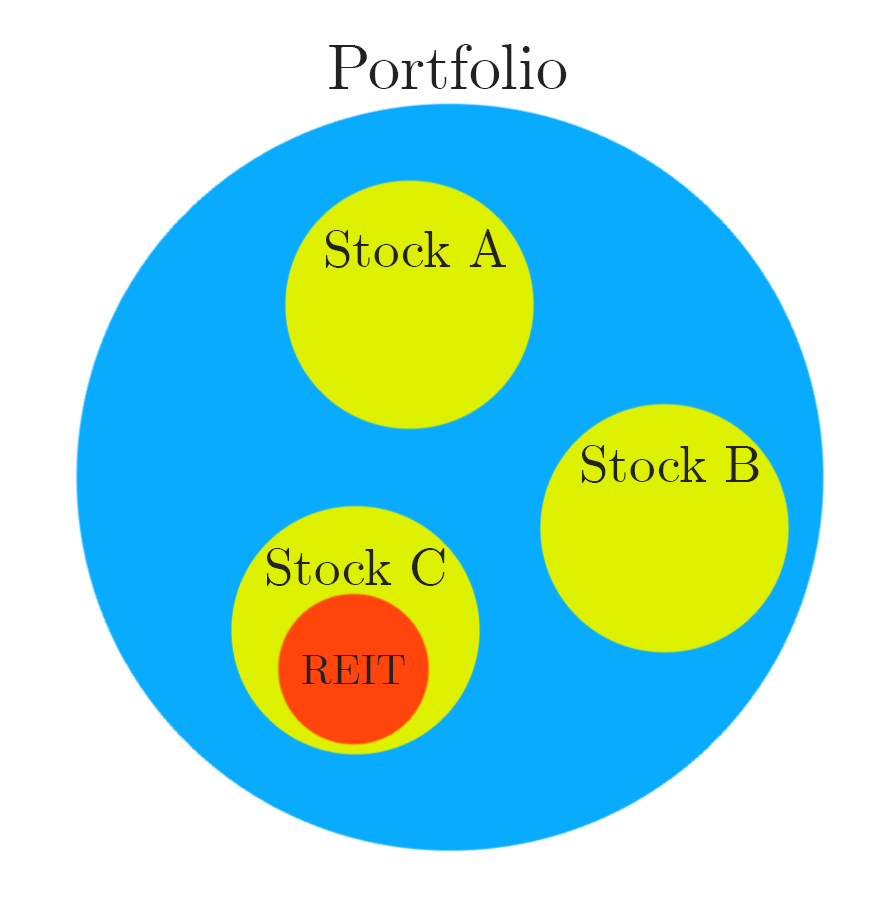
\includegraphics[width=9cm]{Stock_Porfolio_Reit}}
  \caption{Stock vs REIT vs Portfolio}\label{visina8}
  \label{fig:Stock_Porfolio_Reit}
  \end{figure}
\subsection{Stock}
A stock also called a share, represents ownership over a company's assets. Each stock is represented in the market by a unique identifier called a ticker. For instance, Apple's ticker is "AAPL". The proportion ownership depends on how many shares are owned out of the total number of shares in the market and stocks of publicily listed companies can be purchased on the stock exchange. Over time, share prices can rise and fall, and owners can receive a share of the company's profits through dividends. The daily movement of the share prices over time will be represented in this paper by the formula:

\begin{itemize}

  \item {Prices: P is the price of a specific stock at a particular time}
  \item {Date: T in this paper is the daily date}
  \item {Ticker: i is the stock ticker for a specific stock}
  
\end{itemize}
\begin{equation*}
  \overrightarrow{P}\textsubscript{i,1:T} =  
  \begin{bmatrix}
    p\textsubscript{i,1} \\
    p\textsubscript{i,2} \\
    \vdots \\
    p\textsubscript{i,T} \\
  \end{bmatrix}
  \in \mathbb{R}_+^{T}
\end{equation*}

\subsection{Real Estate Investment Trusts (REITs)}
A REIT company invests in properties. Typically these companies invest or own a mix of housing, commercial or industrial properties. Buying shares of REITs allow investors to own a share of the real estate that these REITS are managing and indirectly invest their monies in the real estate sector. Of course, each of the 893 REITs are different companies which own a wide range of different properties across the world. In this paper, a REIT is used to refer to the stock of a REIT company. A REIT is a type of stock.

\subsection{Portfolio}
A portfolio is a collection of stocks i.e a portfolio is a combination of more than one stock. For example, the portfolio in Figure ~\ref{fig:Stock_Porfolio_Reit} consists of 10\% of stock A, 11\% of stock B and 9\% of stock C. The relative proportions of each stock in a portfolio can be represented by weights. This paper will represent a portfolio of stocks with the vector and matrix below:
\begin{itemize}

  \item {Weight: W is the percentage value of a ticker in the portfolio.}
  
\end{itemize}

\begin{equation*}
  \overrightarrow{W}\textsubscript{i,1:T}\overrightarrow{P}\textsubscript{i,1:T} = 
  \begin{bmatrix}
    \overrightarrow{W}\textsubscript{1,1:T}\overrightarrow{P}\textsubscript{1,1:T},\;
    \overrightarrow{W}\textsubscript{2,1:T}\overrightarrow{P}\textsubscript{2,1:T},\;
    \ldots,\;
    \overrightarrow{W}\textsubscript{i,1:T}\overrightarrow{P}\textsubscript{2,1:T}
  \end{bmatrix}
\end{equation*}

\begin{equation*}
= 
  \begin{bmatrix}
    w\textsubscript{1,1}\:p\textsubscript{1,1},&
    w\textsubscript{2,1}\:p\textsubscript{2,1},&
    \ldots,&
    w\textsubscript{i,1}\:p\textsubscript{i,1} 
    \\
    w\textsubscript{1,2}\:p\textsubscript{1,2},&
    w\textsubscript{2,2}\:p\textsubscript{2,2},&
    \ldots,&
    w\textsubscript{i,2}\:p\textsubscript{i,2}
    \\
    \vdots&\vdots&\ddots&\vdots
    \\
    w\textsubscript{1,T}\:p\textsubscript{1,T},&
    w\textsubscript{2,T}\:p\textsubscript{2,T},&
    \ldots,&
    w\textsubscript{i,T}\:p\textsubscript{i,T}
  \end{bmatrix}
  \in \mathbb{R}_+^{M x T}
\end{equation*}
\\
As with prices, the weights of each stock ticker can change daily if the value of the portfolio is redistributed. Depending on the weights assigned and what stocks are in the portfolio, the total portfolio value can change rise or fall. The decision of which stocks to select as part of a portfolio and how much of each stock to buy or hold at every point in time is the central idea of portfolio optimisation. This paper seeks to develop an effective model to select stocks and determine these weights.

\subsection{Shorting}
Conventionally, we need to own a certain stock before we can sell it. However, market makers also allow investors to borrow stocks to sell them first, with the contractual obligation for the investor to repurchase the stocks from the market at a later date to return to the market maker. This mechanism of selling first and buying back later is called shorting and is represented by a negative weight. This paper's analysis allows shorting.


\section{Evaluating Investments with Data}
In this subsection, various measures of investment performance and how they are applied in the paper are discussed. It covers the two main schools of thought in investment analysis, technical and fundamental analysis before discussing Alpha formulas.

\subsection{Technical Analysis with Price Volume Data}
Technical analysis is one method of evaluating investments in stocks and identifying prospective stocks to invest in. It focusses primarily on identifying short term trends in price and volume data. Table \ref{table:technical_data} provides the key features required for technical analysis.

\begin{table}[H]
  \centering
  \caption{Daily Price Volume Data for ticker PLD}
  \begin{tabular}{@{} l *{5}{S[table-format=-1.7]} @{}} 
  \toprule
  {Date} & {Open} & {High} & {Low} & {Close} & {Volume}\\ % center-set header entries
  \midrule
  31/08/2023    &  125.36  & 125.91 &  123.89 &  124.2 & 3277600\\
  01/09/2023   &  125.4  & 125.57 &  124.05 &  124.59 & 1591000\\
  05/09/2023 &  125.36  & 125.91 &  123.89 &  122.05 & 2854100\\
  \bottomrule
  \end{tabular}
  \label{table:technical_data}
\end{table}

\begin{itemize}

  \item {Open: The price of the stock at the start of a trading day}
  \item {High: The highest price of the stock in a trading day}
  \item {Low: The lowest price of the stock in a trading day}
  \item {Close: The price of the stock when the market closes for the day}
  \item {Volume: The total number of shares traded throughout the day}
  
\end{itemize}
The features Open, High, Low and Close are derived from the Price of a stock at different points in the day and trends of these features can indicate future movements, while volume signals the strength of a price trend.

\subsubsection{Profit and Loss (PnL)}
Profits from the purchase of a single stock arises when the selling price of the stock is greater than the original purchase price. However, if the share price falls below the original purchase price then a loss is incurred. Profit or Loss is given by the formula: 
\begin{equation*}
  Profit/Loss = Current Price \times Quantity - Purchase Price \times Quantity
\end{equation*}

\pgfplotstableread{2.pnlDay1.dat}\datatable
\pgfplotstableread{2.pnlDay3.dat}\datatable
\begin{figure}[H]
  \centering
  \centerline{Prices and Profits from Stock A, Purchasing on Different Days}
  \par\medskip
  \begin{subfigure}{.475\linewidth}
    \centering
  \begin{tikzpicture}
  \begin{axis}[
    small,
    xlabel=Day,
    ylabel=\$,
    legend style={at={(0.5,-0.3)},anchor=north},
    smooth,
    ]
  \addplot[mark=*,blue] table [x=Day, y=$SharePrice$]{2.pnlDay1.dat};
  \addlegendentry{$SharePrice$ series}
  \addplot[mark=x,green] table [x=Day, y=$Profit$]{2.pnlDay1.dat};
  \addlegendentry{$Profit$ series}
  \end{axis}
  \end{tikzpicture}
  \caption{Day 1 Purchase}
  \label{graph: prices_and_profits}
\end{subfigure}%
\hfill%
\begin{subfigure}{.475\linewidth}
  \centering
  \begin{tikzpicture}
    \begin{axis}[
      small,
      xlabel=Day,
      ylabel=\$,
      legend style={at={(0.5,-0.3)},anchor=north},
      smooth,
      ]
    \addplot[mark=*,blue] table [x=Day, y=$SharePrice$]{2.pnlDay3.dat};
    \addlegendentry{$SharePrice$ series}
    \addplot[mark=x,red] table [x=Day, y=$Profit$]{2.pnlDay3.dat};
    \addlegendentry{$Profit$ series}
    \end{axis}
    \end{tikzpicture}
    \caption{Day 3 Purchase}
    \label{graph: prices_and_profits2}
  \end{subfigure}
  \caption{}
  \label{figure: prices_and_profits_main}
\end{figure}

It's important to note that profits or losses are only realised when the closing transaction is made i.e. when the stock is sold. Figure \ref{figure: prices_and_profits_main} illustrates that buying the same stock on day 1 versus day 3 can have vastly different results. \\

When a stock is shorted, a rise in price will result in a loss because it becomes more expensive for the investor to repurchase the share. Hence, for shorting the Profit or Loss formula is negated:
\begin{equation*}
  Profit/Loss = -(Current Price \times Quantity - Purchase Price \times Quantity)
\end{equation*}


\subsubsection{Risk and Volatility} \label{Risk and Volatility}
Volatility is a statistical measure of how varied share price and returns on an investment are over a period of time. It is a proxy of the risk of an investment, the likelihood of an investment performing worse than expected. \\
\begin{figure}[H]
  \centering
  \centerline{Prices and Profits from Stock A, Purchasing on Different Days}
  \par\medskip
  \begin{subfigure}{.475\linewidth}
    \centering
    \pgfmathdeclarefunction{gauss}{2}{%
            \pgfmathparse{1/(#2*sqrt(2*pi))*exp(-((x-#1)^2)/(2*#2^2))}%
        }

        \begin{tikzpicture}

        \def\startx{0}    % lower end of domain
        \def\endx{7}       % upper end of domain
        \def\camean{3}  % mean of left side distribution
        \def\casigma{1}  % sigma for left side distribution
        \def\cbmean{3.0}   % mean for right side distribution
        \def\cbsigma{0.5}  % sigma for right side distribution
        \def\verticala{0.7} % x vale for first delimiter
        \def\verticalb{1.3} % x value for second delimited

        \begin{axis}[
        domain=\startx:\endx,
        samples=101,
        ymax=1.2,
        enlargelimits=false,
        axis x line=middle,
        axis y line=middle,
        xtick={0,3},
        xticklabels={0,3},
        ytick={\empty},
        xlabel={$Price$},
        ylabel={$Frequency$},
        height=5cm,
        width=7cm
        ]
        % Draw distributions
        \addplot [name path=a,thin, smooth] {gauss(\camean,\casigma)};
        \addplot [name path=b,thin, smooth] {gauss(\cbmean,\cbsigma)};%    
        % Draw vertical lines:
        %\draw [gray, semithick] (\verticala,0) -- (\verticala,0.4);
        %\draw [gray, semithick] (\verticalb,0) -- (\verticalb,0.4);
        % create path for x axis:
        \path[name path=axis] (axis cs:\startx,0) -- (axis cs:\endx,0);
        % generate fills:
        %\addplot[darkgray]  fill between[of=a and axis,soft clip={domain=\verticala:\verticalb}]; % 
        %\addplot[pattern=north east lines]  fill between[of=b and a,
        %soft clip={(\verticala,0) rectangle (\verticalb,0.5)}
        %]; 
        % place the labels for each distribution
        \node (a) at (3,0.9) {Stock A};
        \node (b) at (5,0.4) {Stock B};

        \end{axis}

        \end{tikzpicture}
        \caption{Price Risk}
        \label{graph: risk_price}
      \end{subfigure}%
      \hfill%
      \begin{subfigure}{.475\linewidth}
      \centering
      \pgfmathdeclarefunction{gauss}{2}{%
            \pgfmathparse{1/(#2*sqrt(2*pi))*exp(-((x-#1)^2)/(2*#2^2))}%
        }

        \begin{tikzpicture}

        \def\startx{0}    % lower end of domain
        \def\endx{7}       % upper end of domain
        \def\camean{3}  % mean of left side distribution
        \def\casigma{1}  % sigma for left side distribution
        \def\cbmean{2.0}   % mean for right side distribution
        \def\cbsigma{0.5}  % sigma for right side distribution
        \def\verticala{0.7} % x vale for first delimiter
        \def\verticalb{1.3} % x value for second delimited

        \begin{axis}[
        domain=\startx:\endx,
        samples=101,
        ymax=1.2,
        enlargelimits=false,
        axis x line=middle,
        axis y line=middle,
        xtick={0,3},
        xticklabels={0,3},
        ytick={\empty},
        xlabel={$Return$},
        ylabel={$Frequency$},
        height=5cm,
        width=7cm
        ]
        % Draw distributions
        \addplot [name path=a,thin, smooth] {gauss(\camean,\casigma)};
        \addplot [name path=b,thin, smooth] {gauss(\cbmean,\cbsigma)};%    
        % Draw vertical lines:
        \draw [gray, semithick] (2,0) -- (2,1);
        \draw [gray, semithick] (3,0) -- (3,0.7);
        % create path for x axis:
        \path[name path=axis] (axis cs:\startx,0) -- (axis cs:\endx,0);
        % generate fills:
        %\addplot[darkgray]  fill between[of=a and axis,soft clip={domain=\verticala:\verticalb}]; % 
        %\addplot[pattern=north east lines]  fill between[of=b and a,
        %soft clip={(\verticala,0) rectangle (\verticalb,0.5)}
        %]; 
        % place the labels for each distribution
        \node (a) at (3,0.9) {Stock A};
        \node (b) at (4,0.5) {Stock B};

        \end{axis}
        
        \end{tikzpicture}
        \caption{Return Risk}
    \label{graph: risk_returns}
  \end{subfigure}
  \caption{}
  \label{figure: risk_volatility_main}
\end{figure}

Figure \ref{graph: risk_price} shows the distribution of prices of Stocks A and B over a period of time. Stock A has a lower standard deviation $\sigma_A$ than Stock B $\sigma_B$, lower volatility and lower price risk.  The returns on both stocks can also be plotted on a similiar distribution as shown in Figure \ref{graph: risk_returns}. Because this paper seeks to minimise risk, the variance of prices and returns need to be considered.

\subsubsection{Sharpe Ratio}
Deciding between stocks or portfolios with different expected returns and risk like in Figure \ref{graph: risk_returns} where Stock B has higher returns but also higher risk than Stock A, requires a formula that evaluates these two measures together. The sharpe ratio combines both measures of profit/loss and risk into a single formula as follows:
\begin{equation*}
  Sharpe Ratio = \frac{R\textsubscript{p}-R\textsubscript{f}}{\sigma\textsubscript{p}}
\end{equation*}
\begin{itemize}
  \item {$R_p$: The annualised return of portfolio}
  \item {$R_f$: The risk free rate}
  \item {$\sigma_p$: The standard deviation of portfolio return}
\end{itemize}
The risk free rate $R_f$ is the return from a zero risk investment such as government bonds. Hence $R_p - R_f$ gives us the excess returns of the portfolio investment compared to a zero risk investment. $\sigma_p$ measures volatility as covered in section \ref{Risk and Volatility}. 
\\

In this paper, the sharpe ratio is used as the overall measure of performance of the portfolio optimisation models and is incorporated in the various objective functions. 
\subsection{Fundamental Analysis with Financial Statements}
Fundamental analysis is a second method of investment analysis that is widely used by finance practitioners but less often applied by Machine Learning researchers. It involves examining the assets and incomes of the companies behind the different stock tickers by looking at their financial statements to evaluate the intrinsic value of a stock. 
\begin{figure}[H]
  \centerline{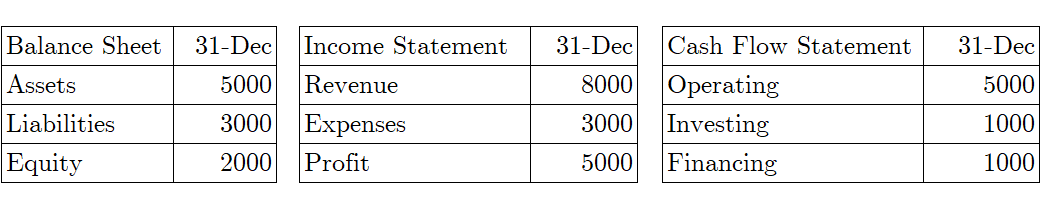
\includegraphics[width=17cm]{financial_statements}}
  \caption{Highly Abbreviated 3 Main Statements}
  \label{fig:financial statements}
\end{figure}
Every quarter, every company with a stock ticker will publish its financial statements which consists of the Balance Sheet, Income Statement and Cash Flow Statement. Figure \ref{fig:financial statements} is a highly abbreviated example, the real financial statements breaks down each category into hundreds of subcategories which can be used as features for Machine Learning.\\

The predictive value of each statement is as follows:
\begin{itemize}
  \item {Income Statement: Profitability of the company's business and the rate of growth of its value}
  \item {Balance Sheet: The asset value and financial stability of the company }
  \item {Cash Flow Statement: How cash is generated by the company}
\end{itemize}

Incorporating both technical and fundamental data into machine learning models can provide a more holistic picture to the analysis and better inform these models with an extended set of short, medium and long term features.

\subsection{Alpha Formulas}
According to quant researcher \cite{tulchinsky_finding_2019}, an Alpha is a formula that determines how much capital to allocate to each stock every day. A good alpha allocates capital in a way that results in a high sharpe ratio for the entire portfolio.\\

Here are two examples of alpha formulas used in real-life trading from a paper by \cite{kakushadze_101_2016}: \\

Alpha 1: $(((high * low)^{0.5}) - vwap)$\\

Alpha 2: $((0.25 < (((delay(close, 20) - delay(close, 10)) / 10) - ((delay(close, 10) - close) / 10))) ?
(-1 * 1) : (((((delay(close, 20) - delay(close, 10)) / 10) - ((delay(close, 10) - close) / 10)) < 0) ? 1 :
((-1 * 1) * (close - delay(close, 1)))))$ \\

The first formula Alpha 1 is relatively simple while Alpha 2 is complex. \\

Figure \ref{fig:alpha table} demonstrates how Alpha 1 is applied to portfolio allocation in a stock portfolio of 6 tickers. Every day, each stock ticker will have its own Alpha value in the first green column of Figure, derived by passing the required features as inputs to the alpha formula (e.g. in this case, Alpha 1 requires, High, Low and Volume Weighted Average Price (Vwap)). \\

\begin{figure}[H]
  \centerline{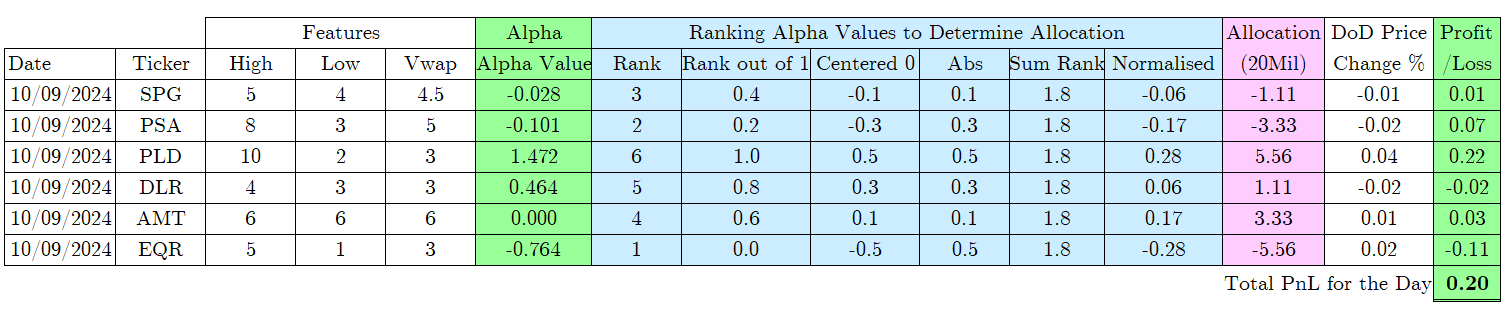
\includegraphics[width=20cm]{alpha_table}}
  \caption{Application of Alpha 1 to Porfolio Allocation}
  \label{fig:alpha table}
\end{figure}

In the blue section of \ref{fig:alpha table}, the Alpha values are then ranked, centered and normalised to determine the relative proportion of the portfolio to allocate to each stock ticker. In a portfolio of 6 tickers, the largest 3 ranks will be bought and the lowest 3 ranks will be shorted to differing degrees. \\

In the pink column, 20 million in capital is allocated by multiplying the total capital of 20 million by the normalised rank. The allocation amount mulitplied by the day-on-day percentage price change (Dod Price Change \%) for each ticker will then give us the Profit/Loss for each stock ticker for the day. The (Dod Price Change \%) formula is as follows:
\begin{equation*}
  (Dod\:Price\:Change\:\%) = \frac{Pave\textsubscript{t+1}-Pave\textsubscript{t}}{|Pave\textsubscript{t}|}
\end{equation*}

\begin{itemize}
  \item {$Pave_{t+1}$: Average of Tommorrow's Open and Close Price}
  \item {$Pave_{t}$: Average of Today's Open and Close Price}
\end{itemize}

The total sum of the Profit/Loss for every ticker is the PnL from the day's investment as all positions are closed and the capital is reallocated the following day. \\

This paper seeks to apply Alpha formulas to allocate REIT portfolios, and go further by developing a Genetic Algorithm inspired by Charles Darwin's theory of evolution to search for strong Alphas to Optimise Real Estate Portfolios. 

\subsection{Other Methods of Analyses}
Sentiment Analysis: Given that share prices in the short run are largely driven by investor sentiment, some researchers have employed Natural Language Processing (NLP) techniques to process trade forum discussions and financial news for trade decision making resulting in good sharpe ratios \cite{alexandria_unlocking_2023}. \\

Macro-economic Analysis: 


\chapter{Literature Review of Portfolio Optimisation Techniques}
\section{Optimal Portfolio Theory}






\begin{landscape}
  \section{Comparison of Traditional and Machine Learning Techniques}

  \begin{table}[H]
    \begin{adjustwidth}{-1.9cm}{-1.9cm}
    \begin{tabular}{|p{2.6cm}|p{2.7cm}|p{2.7cm}|p{3.5cm}|p{5cm}|p{5cm}|p{4cm}|}
    \hline
    \textbf{Methods} & \textbf{Data Inputs} & \textbf{Objectives} & \textbf{Scope for REITs} & \textbf{Strengths} & \textbf{Weaknesses} & \textbf{References}  
    \\ \hline Autoregressive Integrated Moving Average (ARIMA) & Daily Price-Volume Data & Stock Price Prediction and Clustering & Stock Price Prediction & +Suitable for short-term time-series analysis \par+ Widely used in the field of finance for prediction \par+ More explanable than complex ML models & \par-Unsatisfactory for long term prediction \par-Higher RMSE than ML models   & \cite{ariyo_stock_2014},\par \cite{habbab_machine_2022},\par   \cite{obthong_survey_2020}         
    \\ \hline Generalised AutoRegressive Conditional Heteroskedasticity (GARCH) & Daily Commodities Price-Volume data & Stock Volatility Prediction & Stock Volatility Prediction & +Outperforms ARIMA for price prediction and volatility forcasting & - Model assumes volatility can be predicted based on past returns, but volatility in reality is very unpredicatable & \cite{fiszeder_what_2020},   \cite{lama_modelling_2015}, \cite{yuan_garch_2017}           
    \\ \hline Multiple Linear Regression (MLR) & Daily Price-Volume Data & Stock Price Prediction & Stock Price Prediction & +Relatively low RMSE error for stock price prediction \par+ Relatively easy to implement & - Only considers input features and not historical price data  & \cite{obthong_survey_2020}, \cite{shakhla_stock_2020}
    \\ \hline Recurrent Neural Networks (RNN) & Daily Price-Volume Data & Stock Price Prediction & & +Relatively low RMSE error for stock price prediction\par + Remembers historical stock prices & - Susceptible to vanishing and exploding gradient problem & \cite{dey_comparative_2021} 
    \\ \hline Long-Short Term Memory (LSTM) & Daily Price-Volume Data & Stock Price Prediction & Stock Price Prediction & + One of the lowest RMSE error for financial time series prediction \par+ Remembers historical stock prices which are good indicators of future prices \par+ Solves the vanishing and exploding gradient problem & - Mixed results when predicting REIT stock prices & \cite{axelsson_univariate_2023},   \cite{habbab_machine_2022}, \cite{obthong_survey_2020} 
    \\ \hline Random Forest (RF) & Daily Price-Volume Data, Fundamental Data & Stock Price Prediction & & + One of the few papers to incorporate fundamental data into machines learning models & - Relatively low sharpe ratio compared to market indexes & \cite{cao_fundamental_2021},   \cite{huang_machine_2021}  
    \\ \hline Genetic Algorithms & Daily Price-Volume Data & Stock Price Prediction and Clustering & & + Suitable for problems with a large search space \par+ Works well with large time-series data & \cite{obthong_survey_2020}
    \\ \hline
    \end{tabular}
  \end{adjustwidth}
    \end{table}
  




  %\placetextbox{0.5}{0.5}{\fbox{\Huge\textsf{This is my text.}}}%\
  %\placetextbox{0.1}{0.1}{\Large \rotatebox{180}{A}%
\end{landscape}



\subsection{Scope}
\subsection{Profitability}
\subsection{Predictive Accuracy}

\titleformat{\chapter}[block]
  {\normalfont\huge\bfseries}{\thechapter.}{1em}{\Huge\centering}
\titlespacing*{\chapter}{0pt}{150pt}{0pt}
\setcounter{chapter}{1}
\renewcommand{\thechapter}{\Roman{chapter}}
\chapter{Innovation}

\titleformat{\chapter}[display]{\Large}{\centering
  \MakeUppercase{\chaptername}\quad{\Huge\thechapter}}{0pt}{\titlerule[.5pt]\vspace{10pt}\centering
  \MakeUppercase}[\vspace{10pt}{\titlerule[.5pt]}]% <-- spacing of title bar
\titlespacing{\chapter}{0pt}{-80pt}{1cm}% <-- spacing of title bar
\renewcommand{\thechapter}{\arabic{chapter}}
\setcounter{chapter}{3}
\pagenumbering{arabic}
\chapter{Datasets}
\section{Extended Fundamental Data Features}
\section{Feature Selection with Decision Trees}

\def\fillandplacepagenumber{%
 \par\pagestyle{empty}%
 \vbox to 0pt{\vss}\vfill
 \vbox to 0pt{\baselineskip0pt
   \hbox to\linewidth{\hss}%
   \baselineskip\footskip
   \hbox to\linewidth{%
     \hfil\thepage\hfil}\vss}}


\chapter{Methodology}

\begin{figure}[H]
\centerline{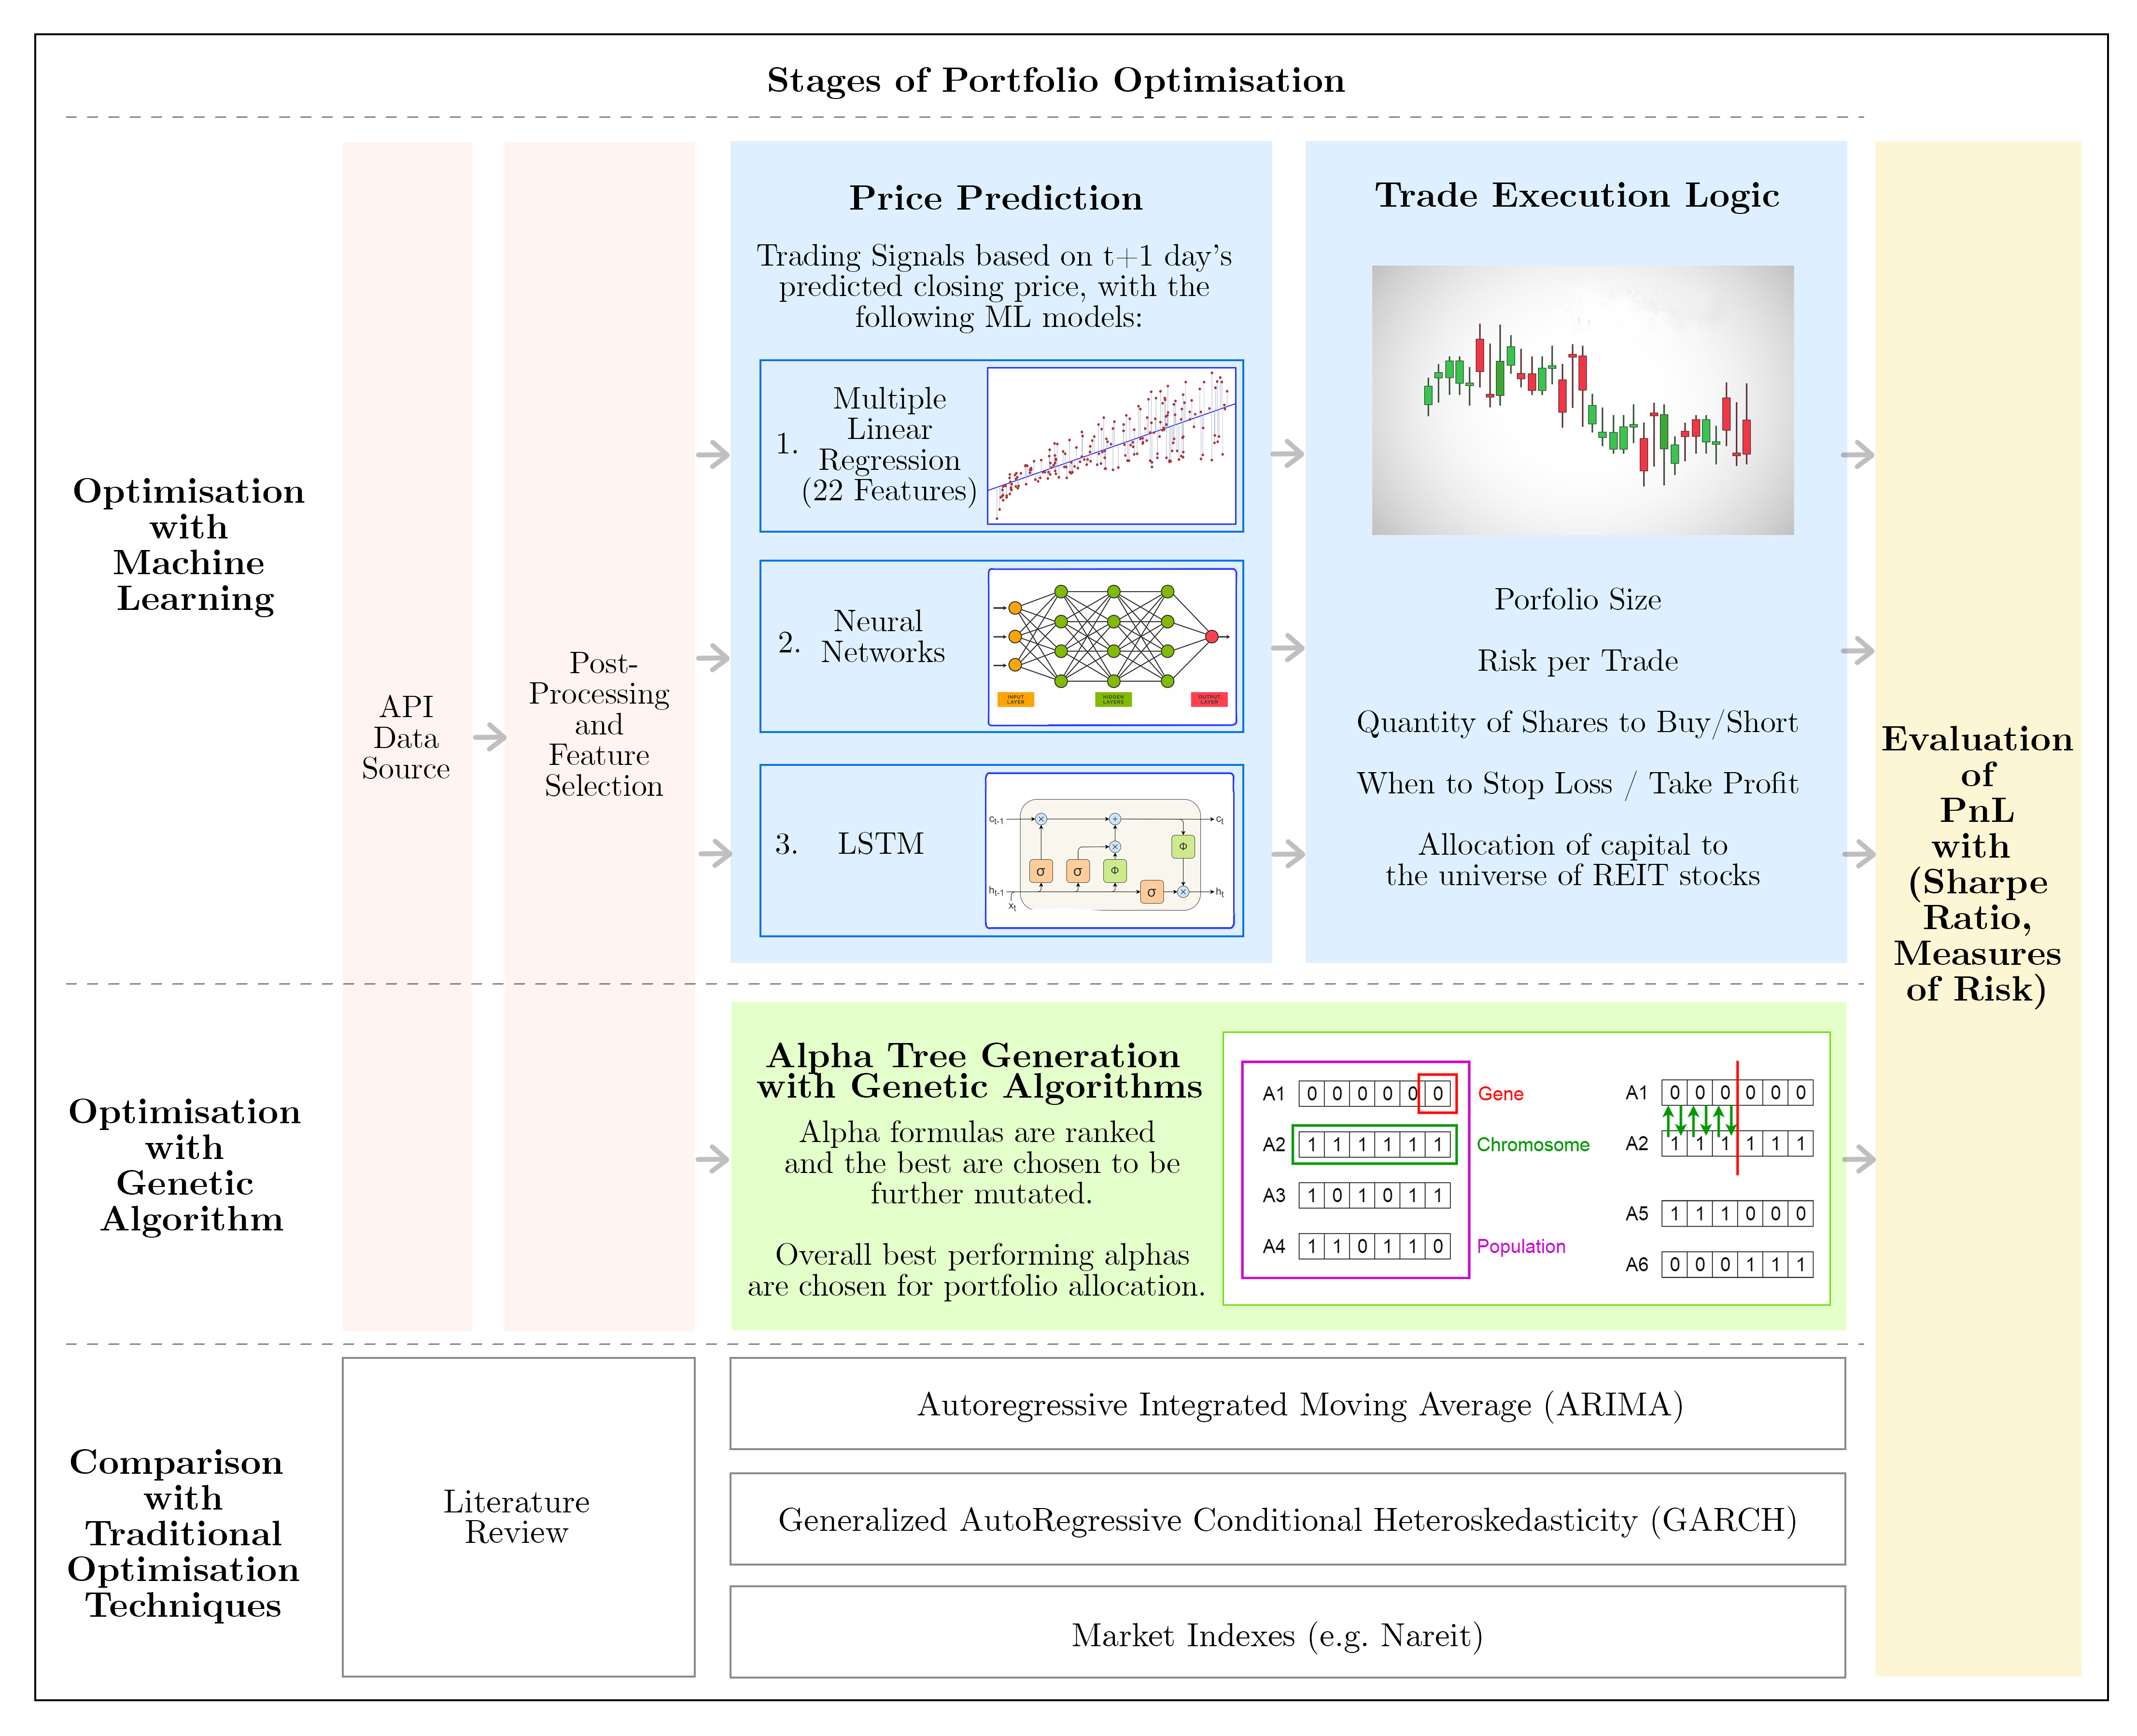
\includegraphics[width=21cm]{Overall_Methodology}}
\caption{Write some caption here}\label{visina8}
\end{figure}


%\begin{landscape}
%\fillandplacepagenumber
%\end{landscape}

\section{Machine Learning for REITs Portfolio Optimisation}
\subsection{MLR / NN / LSTM Predictions with Extended Features}
\subsection{Trade Execution Logic}
\subsection{Performance Evaluation}
\section{Genetic Algorithm Search for Outperforming Alphas}
\subsection{Alpha Tree}
\subsection{Application of Genetic Algorithms to Alpha Trees}
\subsubsection{Objective Function}
\subsubsection{Selection}
\subsubsection{Crossover}
\subsubsection{Mutation}
\subsection{Portfolio Allocation Using Alpha}
\subsection{Performance Evaluation}

\titleformat{\chapter}[block]
  {\normalfont\huge\bfseries}{\thechapter.}{1em}{\Huge\centering}
\titlespacing*{\chapter}{0pt}{150pt}{0pt}
\setcounter{chapter}{2}
\renewcommand{\thechapter}{\Roman{chapter}}
\chapter{Experiments}

\titleformat{\chapter}[display]{\Large}{\centering
  \MakeUppercase{\chaptername}\quad{\Huge\thechapter}}{10pt}{\titlerule[.5pt]\vspace{10pt}\centering
  \MakeUppercase}[\vspace{10pt}{\titlerule[.5pt]}]% <-- spacing of title bar
\titlespacing{\chapter}{0pt}{-23pt}{1cm}% <-- spacing of title bar
\renewcommand{\thechapter}{\arabic{chapter}}
\setcounter{chapter}{5}
\pagenumbering{arabic}
\chapter{Post-processed Financial Datasets}

\chapter{Machine Learning Results}
\section{Evaluating Stock Price Predictions}
\subsection{Multiple Linear Regression (MLR)}
\subsection{Neural Networks (NN)}
\subsection{Long-Short Term Memory (LSTM)}
\section{Trade Execution Results with Different Parameters}
\section{Overall Evaluation of Performances}

\chapter{Alpha Tree Search Results}
\section{Alphas Generated}
\subsection{Initial Set}
\subsection{Intermediate Alphas}
\subsection{Best Performing Alphas}
\section{Portfolio Allocation Results with Best Performing Alphas}
\section{Overall Evaluation of Performance}


\chapter{Conclusion}
\section{Benchmarking Against Index Funds}
\section{Comparing Results with Literature Review}
\section{Key Findings}
\section{Major Contribution and Creativity}
\section{Future Work}
\subsection{More Operators and Features for Alphas}

\begin{figure}[h!]
\centering

\includegraphics[scale=1.7]{universe}
\caption{The Universe}
\label{fig:universe}
\end{figure}


\bibliographystyle{plain}
\bibliography{references}

\end{document}


